\section{Amyotrofisk lateral sklerose} \label{sec:ALS}
ALS er en neurodegenerativ sygdom, der påvirker motorneuronerne i hjernen, hjernestammen og rygsøjlen i takt med sygdommens fremskriden, hvilket resulterer i muskelsvaghed \citep{henschke2012}. 
En illustration af, hvordan ALS påvirker motorneuroner, illustreres på \autoref{fig:affectedneuron}. 
De første symptomer på sygdommen er kramper, svaghed samt stive muskler, hvilket kan opstå som muskelsvaghed i arme eller ben, talebesvær eller svaghed i de muskler, som styrer respirationen \citep{nationalinstitute2016}. 
Symptomer og følger af ALS varierer fra patient til patient, hvorved nogle patienter først oplever muskelsvaghed i deres ben, mens andre oplever muskelsvaghed i deres hænder og arme eller besvær ved tale- eller synkebesvær \citep{nationalinstitute2016, miller2005}.

\begin{figure}[H]
\centering
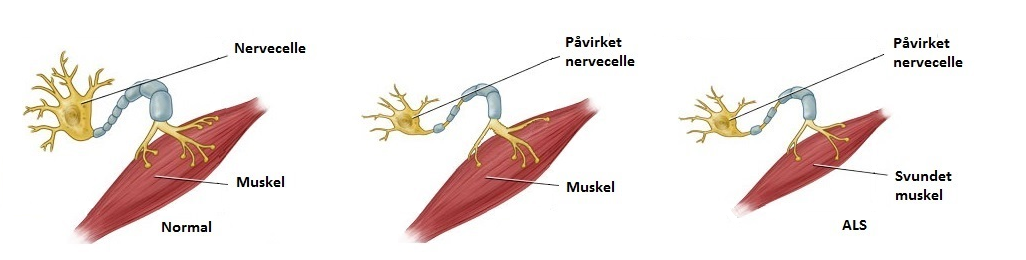
\includegraphics[width=1\textwidth]{figures/affectedneuron}
\caption{Nervecelle og muskel påvirket af ALS. Til venstre ses en normal motorneuron samt en upåvirket muskel. I midten fremgår motorneuronet påvirket af ALS, dog ses musklen endvidere upåvirket. Til højre ses motorneuronet påvirket, samt at musklen er svundet ind. Svindet skyldes en manglende stimulering af musklen som følge af den påvirkede motorneuron \citep{drake2015}.}
\label{fig:affectedneuron}
\end{figure}
 
\noindent
Muskelsvagheden skyldes abnormiteter i de nedre motorneuroner. De nedre motorneuroner er de nerveceller, der videregiver information fra rygmarven til musklerne. 
Symptomer på abnormiteter i de nedre motorneuroner ses som muskelsvaghed samt muskelkramper og atrofi.
Ligeledes kan de øvre motorneuroner påvirkes. Disse motorneuroner sørger for kommunikationen mellem hjernen og de nedre motorneuroner i rygmarven. 
Ved abnormitet, opstår komplikationer ved vidersendelse af beskeder til det givne sted. 
Dette ses som spasticitet samt overdrevne reflekser \citep{nationalinstitute2016}. Opdelingen af de nedre samt øvre motorneuroner ses på \autoref{fig:motorneuroner}.

\begin{figure}[H]
\centering
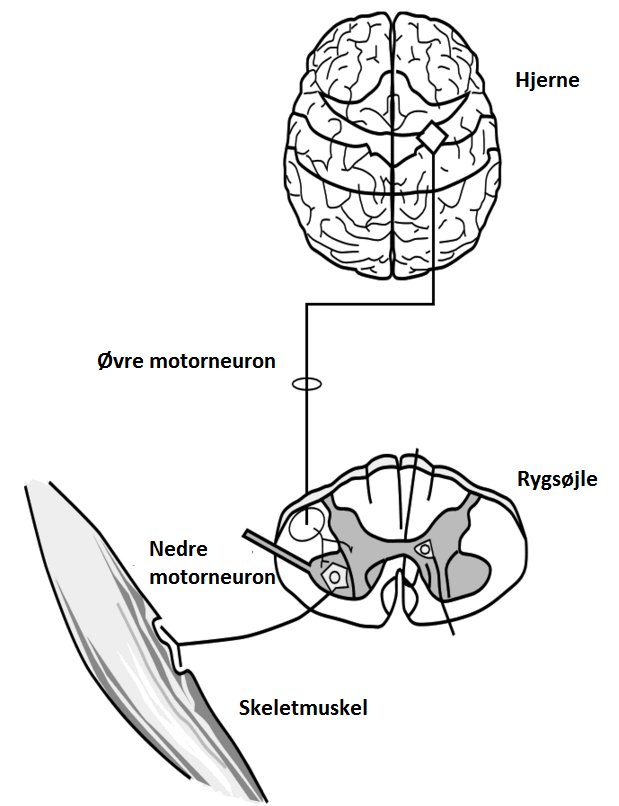
\includegraphics[width=0.6\textwidth]{figures/motorneuroner.png}
\caption{Illustrerer opdelingen af de nedre samt øvre motorneuroner i forhold til hjernen, rygsøjlen og skeletmuskulaturen \citep{miller2005}.}
\label{fig:motorneuroner}
\end{figure}

\noindent
Årsagen til ALS' opståen er oftest ukendt, dog ses en arvelighed i $5 - 10~\%$ af tilfældene. Heraf anslås, at $20~\%$ har det muterede Superocide dismutase 1-gen (SOD-1), hvilket resulterer i tab af motorneuroner \citep{miller2005}.

På trods af, at ALS opleves individuelt både i forhold til sygdomsprogressionen samt, hvilke komplikationer de oplever, kan sygdommen inddeles i tre stadier: et tidligt, midt og endeligt stadie. Et diagram af de tre stadier fremgår af \autoref{fig:stadier}.

\begin{figure}[H]
\centering
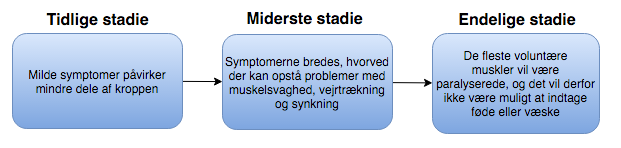
\includegraphics[width=1\textwidth]{figures/stadier.png}
\caption{Tre stadier for udviklingen af ALS samt de tilhørende symptomer.}
\label{fig:stadier}
\end{figure}

\noindent
I det tidlige stadie kan patienter overse symptomer på ALS, da disse er milde og kun påvirker mindre dele af kroppen \citep{themusculardystrophyassociation2016}. 
Ved det midterste stadie vil symptomerne udbrede sig, og nogle muskler paralyseres. Andre muskler vil blive svagere med tiden, hvilket blandt andet kan medføre problemer med synkning og vejrtrækningen \citep{themusculardystrophyassociation2016}. I det endelige stadie vil de fleste voluntære muskler være paralyserede, og det vil derfor forringe muligheden for selv at indtage føde eller væske. 
Herudover vil patienter oftest i dette stadie miste evnen til selv at trække vejret, og de bliver derfor afhængige af ventilationsstøtte \citep{themusculardystrophyassociation2016}.
Den mest almindelige dødsårsag er respirationssvigt, hvilket oftest sker inden for tre til fem år efter diagnosen er stillet \citep{morris2015}. $25~\%$ af patienterne har en overlevelsesrate på fem år, og kun $10~\%$ lever længere end ti år efter diagnosen er stillet \citep{grehl2011, miller2005}.


%Til at starte med kan mindre symptomer som besvær ved at gå op ad trapper opstå. Ligeledes kan patienterne være påvirket af dropfod, når de går. Herefter vil musklerne gradvist blive svagere, og med tiden vil patienterne ikke længere være i stand til at gå.\citep{tidy2015} 